\documentclass{assignment}
\usepackage{amsmath}
\usepackage{graphicx}
\usepackage{hyperref}
\usepackage{listings}
\usepackage{amsmath,bm}
\usepackage{amssymb}
\usepackage{float}
\usepackage{multirow}
\usepackage{pythonhighlight}
\lstset{
numbers=left
}

\coursetitle{Web Mining and Recommender Systems}
\courselabel{CSE 258}
\exercisesheet{Homework Two}{}
\student{Zhang, Jinhan PID A53211930}
\university{University of California, San Diego}
\semester{Winter 2017}
\date{February 5, 2017}

\begin{document}
\begin{problemlist}




\pbitem Solution


\begin{table}[h]
Results after we re-shuffle the data are shown as Table 1:

\vspace{2ex}
\centering
\caption{Results after randomly re-shuffling the data}
\vspace{1ex}

\begin{tabular}{|c|c|c|c|}
\hline
$\lambda$ & Train Accuracy & Validate Accuracy & Test Accuracy \\
\hline
0 & 0.751225490196 & 0.757501530925 & 0.738518064911  \\
\hline
0.01 & 0.748774509804 & 0.757501530925 & 0.738518064911  \\
\hline
1 & 0.729166666667 & 0.753827311696 & 0.72933251684 \\
\hline
100 & 0.66237745098 & 0.681567666871 & 0.680342927128  \\
\hline
\end{tabular}
\end{table}


\vspace{2ex}
\begin{center} 
Listing 1: Key code for Prob.1
\end{center}
\begin{python}
random.seed(0)

print "Reading data..."
dataFile = urllib.urlopen("http://archive.ics.uci.edu/ml/machine-learning-databases/wine-quality/winequality-white.csv")
header = dataFile.readline()
fields = ["constant"] + header.strip().replace('"', '').split(';')
featureNames = fields[:-1]
labelName = fields[-1]
lines = [[1.0] + [float(x) for x in l.split(';')] for l in dataFile]
random.shuffle(lines)        ##randomly shuffle
X = [l[:-1] for l in lines]
y = [l[-1] > 5 for l in lines]
print "done"
\end{python}

\vspace{3ex}

\pbitem Solution
\vspace{30ex}
\begin{table}[h]
Classifiers Evaluation Results are shown as Table 2:

\vspace{2ex}
\centering
\caption{Classifiers Evaluation Value}
\vspace{1ex}

\begin{tabular}{|c|c|}
\hline
True Positives & 1129 \\
\hline
True Negatives & 145  \\
\hline
False Positives & 321  \\
\hline
False Negatives & 38 \\
\hline
Balanced Error Rate & 0.360701663412  \\
\hline
\end{tabular}
\end{table}

\begin{center} 
Listing 2: Key code for Prob.2
\end{center}
\begin{python}
def performance2(theta):

    scores_test = [inner(theta, x) for x in X_test]

    predictions_test = [s > 0 for s in scores_test]
    TP = sum([(a == 1 and b == 1) for (a, b) in zip(predictions_test, y_test)])
    TN = sum([(a == 0 and b == 0) for (a, b) in zip(predictions_test, y_test)])
    FP = sum([(a == 1 and b == 0) for (a, b) in zip(predictions_test, y_test)])
    FN = sum([(a == 0 and b == 1) for (a, b) in zip(predictions_test, y_test)])
    TPR = TP * 1.0 / (TP + FN)
    TNR = TN * 1.0 / (TN + FP)
    BER = 1 - (TPR + TNR) / 2

    return TP,TN,FP,FN,BER


lam = 0.01
theta = train(lam)
TP,TN,FP,FN,BER = performance2(theta)
print("TP = " + str(TP) + ";TN=" + str(TN) + "; FP=" + str(FP) + "; FN=" + str(
FN) + "; BER=" + str(BER))
\end{python}

\pbitem Solution

\begin{table}[h]
Results are shown as Table 3:

\vspace{2ex}
\centering
\caption{Ranking Evaluation Results}
\vspace{1ex}

\begin{tabular}{|c|c|c|c|}
\hline
Number of Return & Precision & Recall \\
\hline
10 & 1.0 & 0.00856898029135  \\
\hline
500 & 0.956 & 0.409597257926  \\
\hline
1000 & 0.864 & 0.740359897172 \\
\hline
\end{tabular}
\end{table}

\vspace{17ex}
\begin{center} 
Listing 3: Key code for Prob.3
\end{center}
\begin{python}
def performance3(theta,numR):

    scores_test = [inner(theta, x) for x in X_test]
    combine = [[scores_test[i]] + [y_test[i]] for i in range(0, len(y_test))]
    combine.sort(key=lambda x: x[0], reverse=True)
    total = sum(l[1]==True for l in combine)
    rel = sum(combine[i][1]==True for i in range(0,numR))
    precision = rel * 1.0 / numR
    recall = rel *1.0 / total

    return precision,recall

lam = 0.01
theta = train(lam)
for numReturn in [10,500,1000]:
    precision,recall = performance3(theta,numReturn)
    print("numReturn = " + str(numReturn) + ";\tprecision=" + str(precision) + "; recall=" + str(recall))
\end{python}

\pbitem Solution

Plot is shown as Fig.1 below:
\begin{figure}[H]
\centering
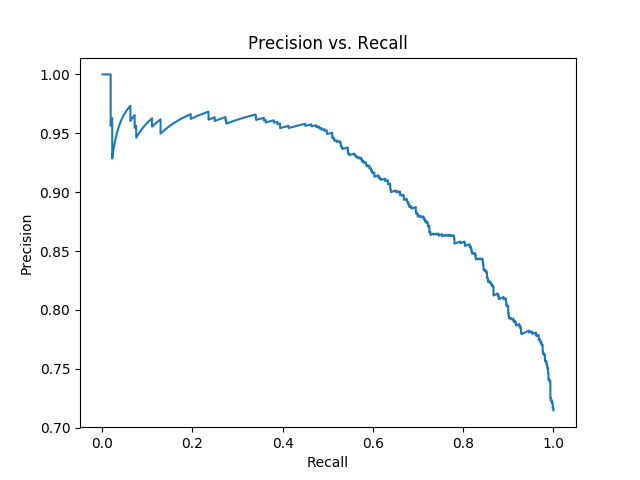
\includegraphics[width=5in]{figure_4}
\caption{Precision vs. recall as the number of results considered varies }
\end{figure}

\begin{center} 
Listing 4: Key code for Prob.4
\end{center}
\begin{python}
def performance3(theta,numR):

    scores_test = [inner(theta, x) for x in X_test]
    combine = [[scores_test[i]] + [y_test[i]] for i in range(0, len(y_test))]
    combine.sort(key=lambda x: x[0], reverse=True)
    total = sum(l[1]==True for l in combine)
    rel = sum(combine[i][1]==True for i in range(0,numR))
    precision = rel * 1.0 / numR
    recall = rel *1.0 / total

    return precision,recall


lam = 0.01
theta = train(lam)
result_pre = []
result_rec = []
for numReturn in range(1,len(y_test)+1):
    precision,recall = performance3(theta,numReturn)
    result_pre.append(precision)
    result_rec.append(recall)
plt.plot(result_rec,result_pre)
plt.xlabel('Recall')
plt.ylabel('Precision')
plt.title('Precision vs. Recall')
plt.show()
\end{python}

\pbitem Solution

The 'reconstruction error' of the naive 'compression' is: 3675818.61688 

\begin{center} 
Listing 5: Key code for Prob.5
\end{center}
\begin{python}
X_mean=numpy.mean(X_train,axis=0)
diff=X_train-X_mean
re=sum(sum(numpy.multiply(diff,diff)).T)
print re
\end{python}

\pbitem Solution
\vspace{2ex}

PCA components of winequality dataset are shown as Fig.2 below:
\begin{figure}[H]
\centering
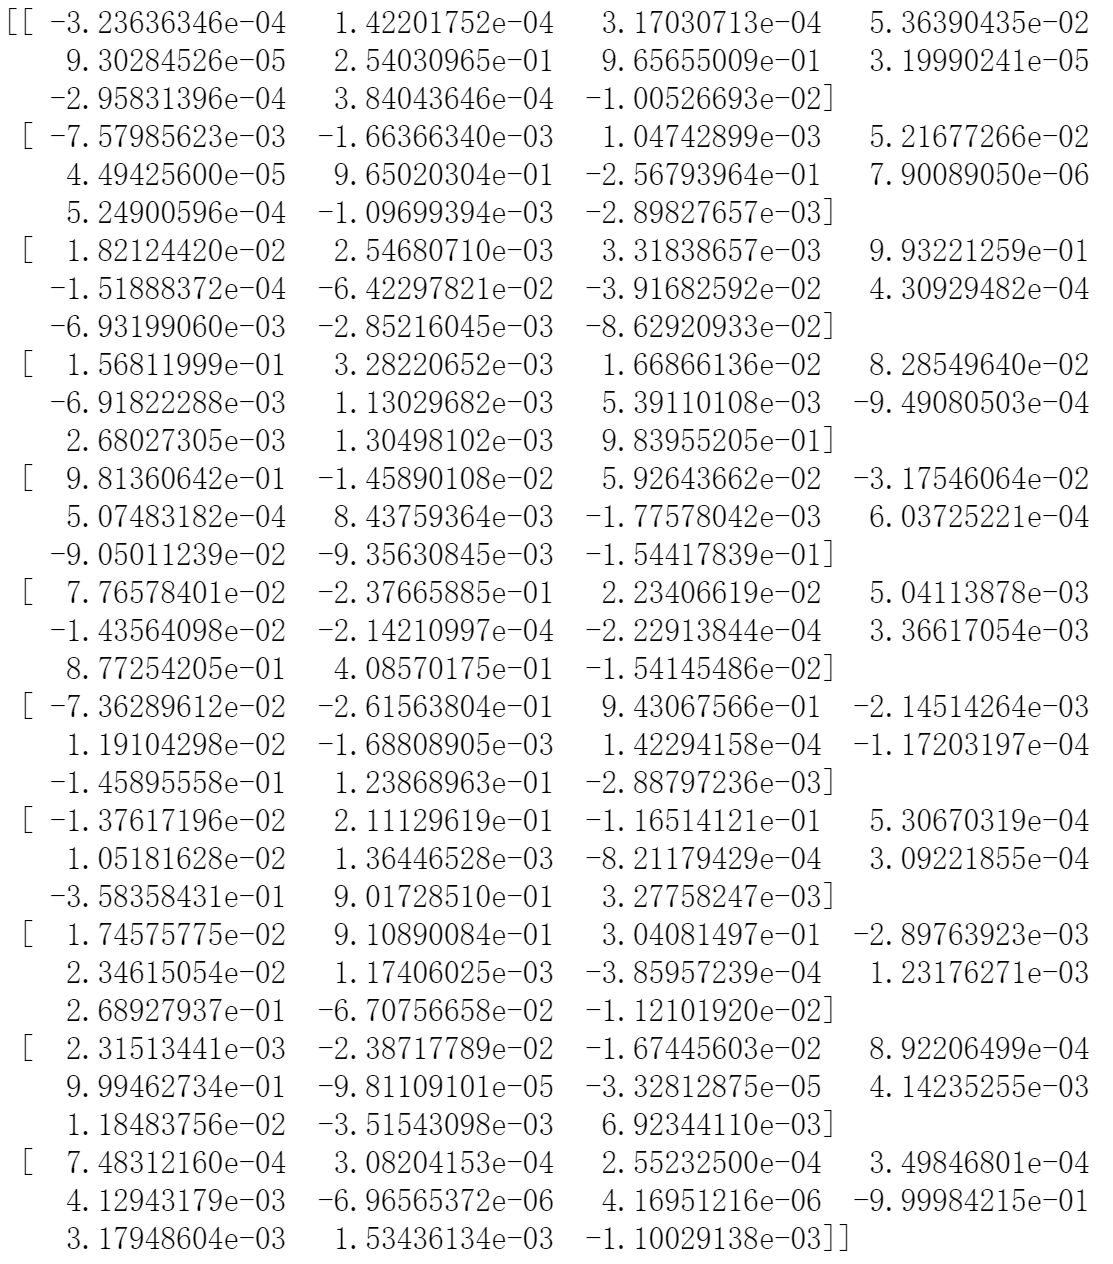
\includegraphics[width=5in]{figure_6}
\caption{PCA components of winequality dataset}
\end{figure}

\begin{center} 
Listing 6: Key code for Prob.6
\end{center}
\begin{python}
print "Reading data..."
dataFile = urllib.urlopen("http://archive.ics.uci.edu/ml/machine-learning-databases/wine-quality/winequality-white.csv")
header = dataFile.readline()
fields = ["constant"] + header.strip().replace('"', '').split(';')
featureNames = fields[:-1]
labelName = fields[-1]
lines = [[float(x) for x in l.split(';')] for l in dataFile]
X = [l[:-1] for l in lines]
y = [l[-1] > 5 for l in lines]
print "done"

X_train = X[:int(len(X) / 3)]
y_train = y[:int(len(y) / 3)]
X_validate = X[int(len(X) / 3):int(2 * len(X) / 3)]
y_validate = y[int(len(y) / 3):int(2 * len(y) / 3)]
X_test = X[int(2 * len(X) / 3):]
y_test = y[int(2 * len(X) / 3):]

pca = PCA(n_components=11)
pca.fit(X_train)
print pca.components_
\end{python}

\pbitem Solution
\vspace{2ex}

The reconstruction error is: 1345.47557409

We can use two ways to compute the reconstruction error, one is to use the projection matrix we get to reconstruct original daata and then compute the error, the other is use the sum of the variance we drop to compute the reconstruction error.

\begin{center} 
Listing 7: Key code for Prob.7
\end{center}
\begin{python}
pca = PCA(n_components=4)
pca.fit(X_train)


X_PCA=pca.fit_transform(X_train)     	##Way 1
x_rec2=pca.inverse_transform(X_PCA)
x_rec2=numpy.matrix(x_rec2)
error2=sum(sum(numpy.multiply(x_rec2-X_train,x_rec2-X_train)).T).tolist()[0][0]
print error2

print pca.noise_variance_*len(x_rec2)   ##Way 2
\end{python}

\pbitem Solution
\vspace{2ex}

Plot is shown as Fig.3 below. We can see from the plot that both training and test set MSE decrease with the increment of the number of dimensions in general. And the test set sometimes gets higher MSE with a higher number of dimensions.

\begin{figure}[H]
\centering
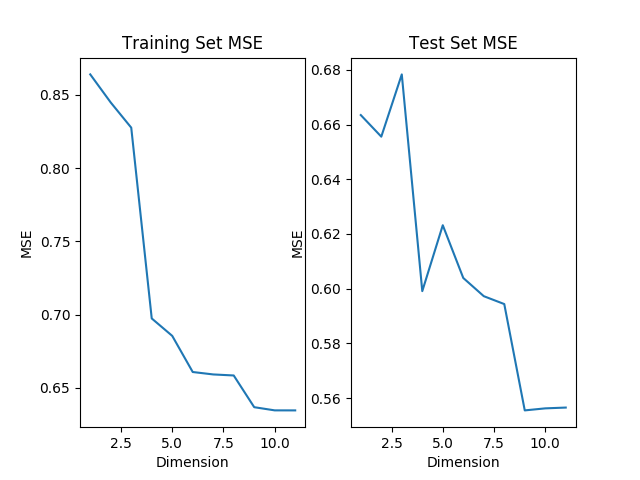
\includegraphics[width=5in]{figure_8}
\caption{ MSE vs. dimensions on the train and test sets}
\end{figure}

\begin{center} 
Listing 8: Key code for Prob.8
\end{center}
\begin{python}
train_mse=[]
test_mse=[]

for dim in range(1,12):
    pca = PCA(n_components=dim)
    X_PCA = pca.fit_transform(X_train).tolist()
    X_PCA = [[1] + elem for elem in X_PCA]
    theta, l, info = scipy.optimize.fmin_l_bfgs_b(f, [0]*(dim+1), fprime, args = (X_PCA, y_train, 0))  #lambda
    #print "Final log likelihood =", -l
    X_test_PCA = pca.transform(X_test).tolist()
    X_test_PCA = [[1] + elem for elem in X_test_PCA]
    X_test_PCA=numpy.matrix(X_test_PCA)
    theta=numpy.matrix(theta)
    y_test=numpy.matrix(y_test)
    y=X_test_PCA*theta.T
    k=y-y_test.T
    mse2=(k.T*k/len(y)).tolist()[0][0]
    test_mse.append(mse2)

    X_PCA = numpy.matrix(X_PCA)
    y_train = numpy.matrix(y_train)
    y = X_PCA * theta.T
    k = y - y_train.T
    mse1 = (k.T * k / len(y)).tolist()[0][0]
    train_mse.append(mse1)
XX=range(1,12)
plt.figure()
ax1 = plt.subplot(121)
ax2 = plt.subplot(122)
plt.sca(ax1)
plt.plot(XX,train_mse)
plt.title('Training Set MSE')
plt.xlabel('Dimension')
plt.ylabel('MSE')
plt.sca(ax2)
plt.plot(XX,test_mse)
plt.xlabel('Dimension')
plt.ylabel('MSE')
plt.title('Test Set MSE')
plt.show()
\end{python}


\end{problemlist}
\end{document}
